\noindent The bridged-T attenuator (Fig. \ref{fig:bridged-tee-attenuator-schematic}) requires $Z_{in}$ and $Z_{out}$ to be equal. The design equations are the following \cite{vizmuller1995rf}:

  \begin{figure}[ht]
    \centering
    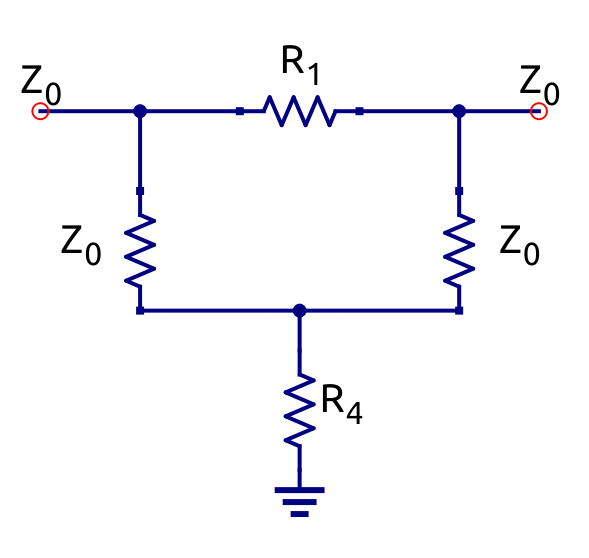
\includegraphics[width=5cm]{./images/bridged-tee-attenuator-schematic.png}
    \caption{Bridged-T attenuator}
    \label{fig:bridged-tee-attenuator-schematic}
  \end{figure}

\begin{equation}
	R_1 = Z_0 \cdot (10^{\alpha/20} - 1)
\end{equation}

\begin{equation}
	R_4 = \frac{Z_0}{10^{\alpha/20} - 1}
\end{equation}
  
\noindent where $\alpha$ is the attenuation in dB. The power dissipation expressions for each resistor are the following:

\begin{equation}
	P_{R1} = P_{in} \cdot \frac{4 \cdot R_1 \cdot R_4^2 \cdot Z_0}{(R_1 \cdot R_4 + Z_0 \cdot (2 \cdot R_4 + Z_0))^2}
\end{equation}

\begin{equation}
	P_{R2} = P_{in} \cdot \frac{(R_1 \cdot R_4 + Z_0^2)^2}{(R_1 \cdot R_4 + Z_0 \cdot (2 \cdot R_4 + Z_0))^2}
\end{equation}

\begin{equation}
	P_{R3} = 0
\end{equation}

\begin{equation}
	P_{R4} = P_{in} \cdot  \frac{4 \cdot R_4 \cdot Z_0^3}{(R_1 \cdot R_4 + Z_0 \cdot (2 \cdot R_4 + Z_0))^2}
\end{equation}

\noindent Fig. \ref{fig:pi-tee-relative-power-dissipation-50-Ohm} shows the power dissipated by each resistor with respect to the input power. Notice that the vast majority of the power is dissipated by $R_2 (= Z_0)$ for attenuations larger than 6 dB.


  \begin{figure}[ht]
    \centering
    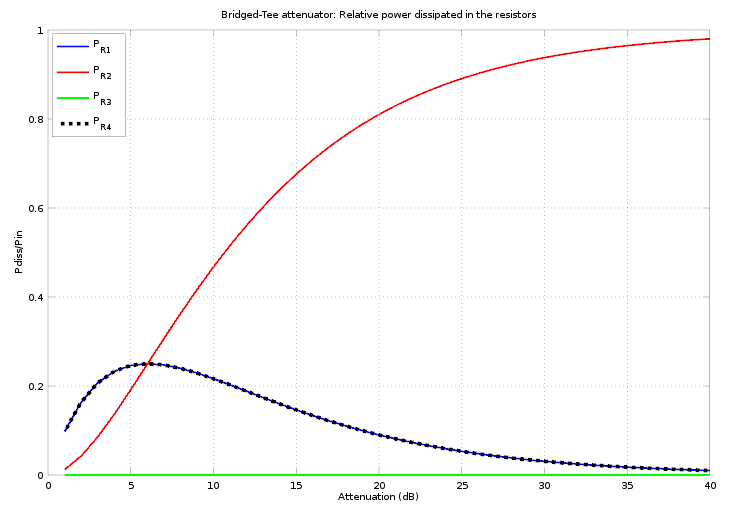
\includegraphics[width=10cm]{./images/bridged-tee-relative-power-dissipation-50-Ohm.png}
    \caption{Power dissipated in the resistor for the bridged-T attenuator with respect to the input power. $Z_{in} = Z_{out} = 50 \Omega$}
    \label{fig:bridged-tee-relative-power-dissipation-50-Ohm}
  \end{figure}